%%%%%%%%%%%%%%%%%%%%%%%%%%%%%%%%%%%%%%%%%%%%%%
% Head matter - can we try to be consistent on
% included packages
\documentclass{beamer}
\mode<presentation>
{\usetheme{default}
 \usecolortheme{default}
 \usefonttheme{default}
 \setbeamertemplate{navigation symbols}{}
 \setbeamertemplate{footline}[frame number]
% \setbeamertemplate{caption}[numbered]
 }
\usepackage[english]{babel}
\usepackage{algorithm}
\usepackage[noend]{algpseudocode}
\usepackage[utf8x]{inputenc}
\usepackage{graphicx}
\usepackage{hyperref}
%\graphicspath{{./images/}}
\usepackage{tikz}
\usetikzlibrary{shapes.geometric, arrows,chains}
\usepackage{booktabs,makecell,multirow,tabularx}
\usepackage{verbatim}
\renewcommand{\arraystretch}{1.2}
\renewcommand\theadfont{\normalfont\bfseries}
\usepackage{array}
\usepackage{listings}
\lstset{language=Java, showstringspaces=false}
\usepackage[normalem]{ulem}
\usepackage{bm}
\def\layersep{2.5cm}

\usepackage{xcolor}
%\usepackage{subfig}
\setbeamertemplate{caption}{\insertcaption}
\usepackage[caption=false]{subfig}
\usepackage{hyperref}
\usepackage{verbatim}
%\setbeamertemplate{caption}[numbered]%\numberwithin{figure}{section}
% Define block styles
\tikzstyle{decision} = [diamond, draw, fill=blue!20, 
    text width=4.5em, text badly centered, node distance=3cm, inner sep=0pt]
\tikzstyle{block} = [rectangle, draw, fill=blue!20, 
    text width=3em, text centered, rounded corners, minimum height=3em]
\tikzstyle{line} = [draw, -latex']
\tikzstyle{cloud} = [draw, ellipse, fill=red!20, node distance=3cm,
    minimum height=2em]
\tikzset{
  startstop/.style={
    rectangle, 
    rounded corners,
    minimum width=3cm, 
    minimum height=1cm,
    align=center, 
    draw=black, 
    fill=red!30
    },
  process/.style={
    rectangle, 
    minimum width=3cm, 
    minimum height=1cm, 
    align=center, 
    draw=black, 
    fill=blue!30
    },
  decision/.style={
    rectangle, 
    minimum width=3cm, 
    minimum height=1cm, align=center, 
    draw=black, 
    fill=green!30
    },
  arrow/.style={thick,->,>=stealth},
  dec/.style={
    ellipse, 
    align=center, 
    draw=black, 
    fill=green!30
    },
}
\tikzstyle{arrow} = [thick,->,>=stealth]

\tikzset{onslide/.code args={<#1>#2}{%
  \only<#1>{\pgfkeysalso{#2}} % \pgfkeysalso doesn't change the path
}}

\makeatletter
\newenvironment<>{btHighlight}[1][]
{\begin{onlyenv}#2\begingroup\tikzset{bt@Highlight@par/.style={#1}}\begin{lrbox}{\@tempboxa}}
{\end{lrbox}\bt@HL@box[bt@Highlight@par]{\@tempboxa}\endgroup\end{onlyenv}}

\newcommand<>\btHL[1][]{%
  \only#2{\begin{btHighlight}[#1]\bgroup\aftergroup\bt@HL@endenv}%
}
\def\bt@HL@endenv{%
  \end{btHighlight}%   
  \egroup
}
\newcommand{\bt@HL@box}[2][]{%
  \tikz[#1]{%
    \pgfpathrectangle{\pgfpoint{1pt}{0pt}}{\pgfpoint{\wd #2}{\ht #2}}%
    \pgfusepath{use as bounding box}%
    \node[anchor=base west, fill=orange!30,outer sep=0pt,inner xsep=1pt, inner ysep=0pt, rounded corners=3pt, minimum height=\ht\strutbox+1pt,#1]{\raisebox{1pt}{\strut}\strut\usebox{#2}};
  }%
}
\makeatother


%%%%%%%%%%%%%%%%%%%%%%%%%%%%%%%%%%%%%%%%%%%%%%
% Formatting for title page
\title[Deep Learning]{Generative Adversarial Networks}
\author{Kate Farrahi}
\institute{ECS Southampton}
\date{\today}
%%%%%%%%%%%%%%%%%%%%%%%%%%%%%%%%%%%%%%%%%%%%%%
\begin{document}
\begin{frame}
  \titlepage
\end{frame}

%-------------------------------------------------------------%
\begin{frame}[fragile]{pause}\frametitle{Generative Modeling}
		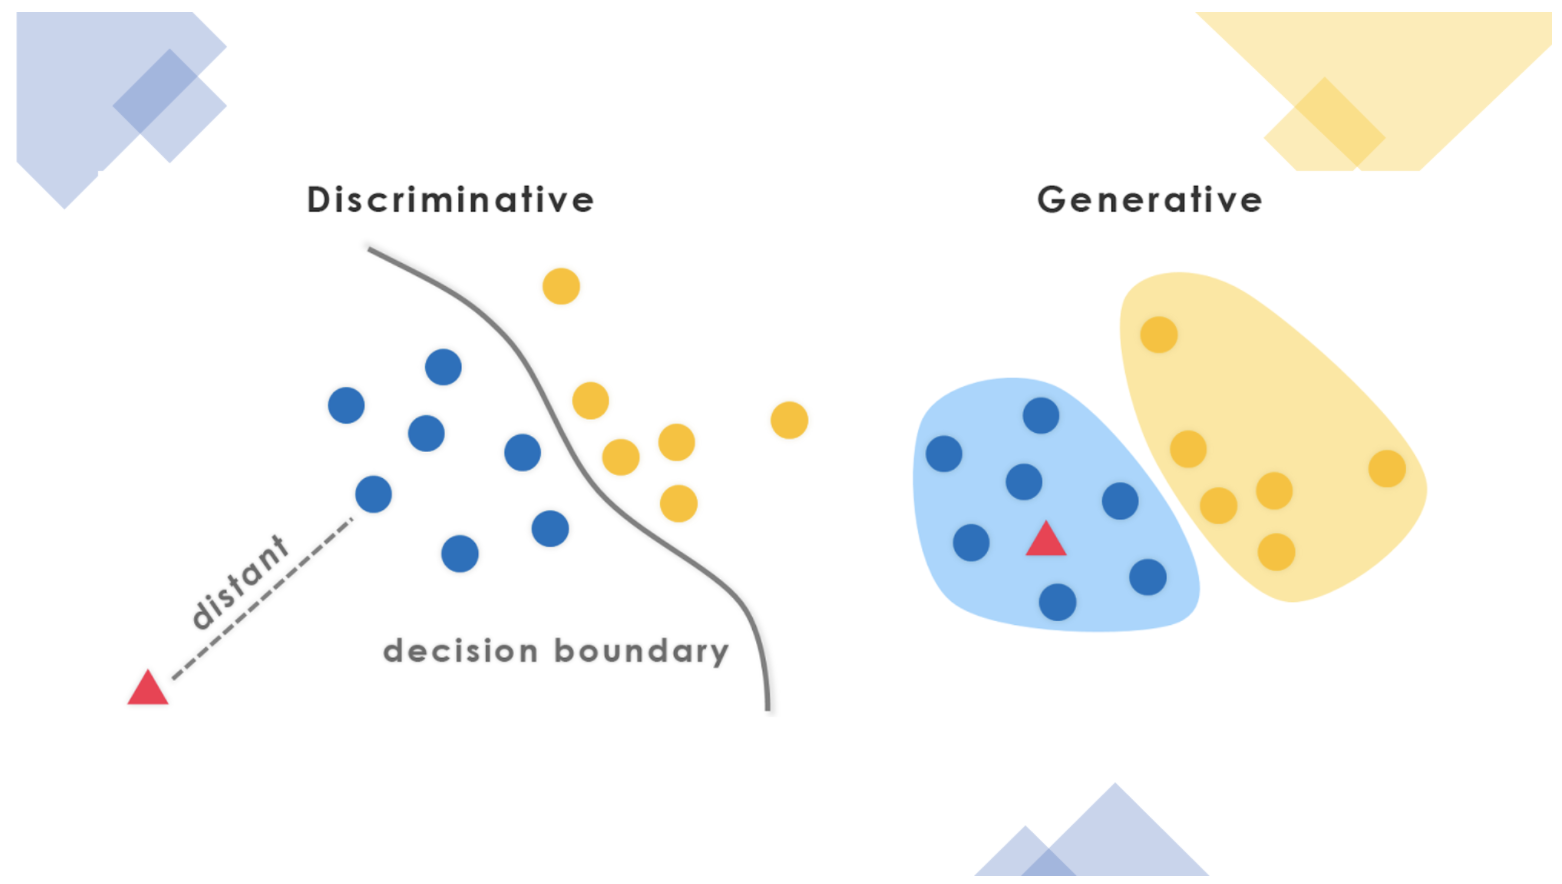
\includegraphics[width=10cm]{figs/generative_modeling.png}\footnote{Image Taken from \url{https://www.kdnuggets.com/2020/05/microsoft-research-three-efforts-advance-deep-generative-models.html}}
	\end{frame}


%-------------------------------------------------------------%
\begin{frame}[fragile]{pause}\frametitle{Generative Modeling}
	
	\begin{itemize}
		\item Can you generate a sample from Normal Distribution? \footnote{\url{https://bjlkeng.github.io/posts/sampling-from-a-normal-distribution/}}
		\item Can you generate an MNIST image?
	\end{itemize}


	\end{frame}

%-------------------------------------------------------------%
\begin{frame}[fragile]{pause}\frametitle{Lecture Outline: Paper References}
\begin{itemize}
\item Paper 1: Goodfellow, Ian, et al. "Generative adversarial nets." Advances in neural information processing systems. 2014. \footnote{\url{https://proceedings.neurips.cc/paper/2014/file/5ca3e9b122f61f8f06494c97b1afccf3-Paper.pdf}}
\item Paper 2: Radford, Alec, Luke Metz, and Soumith Chintala. "Unsupervised representation learning with deep convolutional generative adversarial networks." \footnote{\url{https://arxiv.org/pdf/1511.06434.pdf}}
%\item Paper 3: Arjovsky, Martin, Soumith Chintala, and Leon Bottou. "Wasserstein generative adversarial networks." International Conference on Machine Learning. 2017.
\end{itemize}
\end{frame}
%-------------------------------------------------------------%

\begin{frame}[fragile]{pause}\frametitle{Generative Adversarial Networks (GANs)}
\begin{itemize}
\item New method of training deep generative models \pause
\item Idea: put a generator and a discriminator against each other \pause
%\item Generator tries to draw samples from P(X) \pause
\item Discriminator tries to tell if sample came from the generator (fake) or the real world \pause
\item Both discriminator and generator are deep networks (differentiable functions) \pause
\item LeCun quote "GANs, the most interesting idea in the last ten years in machine learning" \pause
\end{itemize}
\end{frame}

%-------------------------------------------------------------%

\begin{frame}[fragile]{pause}\frametitle{Advantages of VAEs (over GANs)}
	\begin{itemize}
		\item VAEs have a probabilistic formulation as a result of maximizing a lower bound on the log-likelihood.
		
		\item Usually easier to train and get working. 
		
		\item Relatively easy to implement and robust to hyperparameter choices.
		
		\item Tractable likelihood.
		
		\item Has an explicit inference network allowing us to do reconstruction.
		\footnote{ \url{https://www.reddit.com/r/MachineLearning/comments/4r3pjy/variational_autoencoders_vae_vs_generative/}}
	\end{itemize}
\end{frame}

%-------------------------------------------------------------%

\begin{frame}[fragile]{pause}\frametitle{Advantages of GANs (over VAEs)}
	\begin{itemize}

	\item GANs have much higher visual fidelity in generated samples.

	\item GANs are better at generating visual features (adversarial loss is better than mean-squared loss).

	\end{itemize}
\end{frame}

\begin{frame}[fragile]\frametitle{Adversarial Approach vs. Adversarial Examples}
The approach of GANs is called adversarial since the two networks have antagonistic objectives.\\ \vspace{0.5cm}

This is not to be confused with adversarial examples in machine learning. \vspace{0.5cm}

See these two papers for more details: \\
\url{https://arxiv.org/pdf/1412.6572.pdf} \\
\url{https://arxiv.org/pdf/1312.6199.pdf}
\end{frame}
%-------------------------------------------------------------%

\begin{frame}[fragile]
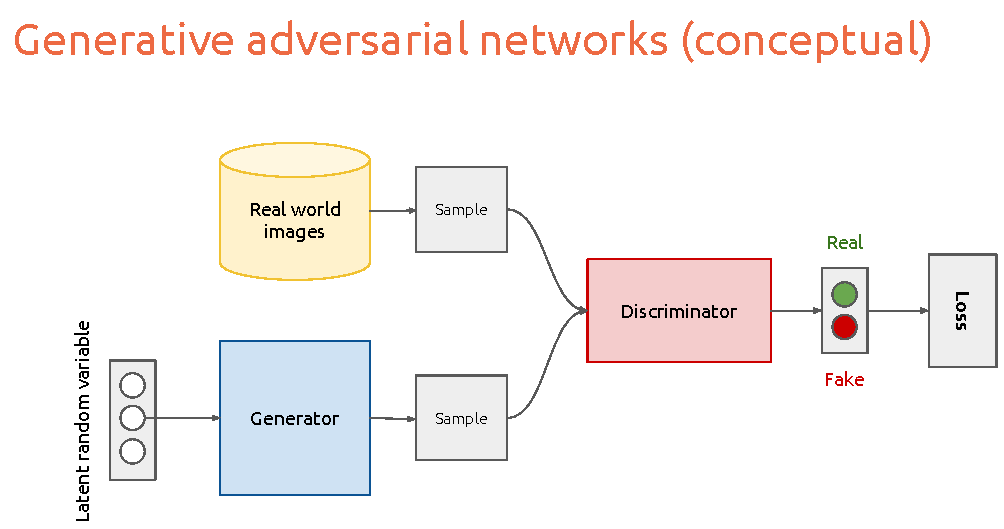
\includegraphics[width=10cm]{figs/GANS_1.pdf} \footnote{Credit: Xavier Giro-i-Nieto}
\end{frame}
%-------------------------------------------------------------%

\begin{frame}[fragile]{pause}\frametitle{More Formally}
\begin{itemize}
\item The {\bf generator}
		\begin{equation}
		{\bf G}:	\mathbb{R}^D \rightarrow X
		\end{equation}
		
		is trained so that it gets a random input and produces a sample following the data distribution as output (ideally). \vspace{1cm}

\item The {\bf discriminator}
	\begin{equation}
	{\bf D}: X \rightarrow [0,1]
	\end{equation}
	gets a sample as input and predicts if it is real or fake.
\end{itemize}
\end{frame}
%-------------------------------------------------------------%

\begin{frame}[fragile]{pause}\frametitle{More Practically}
\begin{itemize}
\item Training a standard GAN is difficult and often results in two undesirable behaviors
\begin{enumerate}
\item Oscillations without convergence. Contrary to standard loss minimization,
we have no guarantee that the loss will actually decrease.
\item The {\bf mode collapse} problem, when the generator models very well a small
sub-population, concentrating on a few modes.
\end{enumerate}
\item Additionally, performance is hard to assess and often boils down to heuristic observations.
\end{itemize}
\end{frame}
%-------------------------------------------------------------%

\begin{frame}[fragile]{pause}\frametitle{Deep Convolutional Generative Adversarial Networks (DCGANs)}
\begin{itemize}
\item Motivates the use of GANS to learn reusable feature representations from large unlabeled datasets. \pause
\item GANs known to be unstable to train, often resulting in generators that produce "nonsensical outputs". \pause
\item Extensive model exploration to identify a family of architectures that result in {\bf stable} training across a range of datasets and allowed for training higher resolution and deeper models. 
\end{itemize}
\end{frame}
%-------------------------------------------------------------%


\begin{frame}[fragile]{pause}\frametitle{Architecture Guidelines for Stable DCGAN}
\begin{itemize}
\item Replace pooling layers with strided convolutions in the discriminator and fractional-strided convolutions in the generator. \pause This will allow the network to learn its own spatial downsampling. \pause
\item Use batchnorm in both the generator and the discriminator. \pause This helps deal with training problems due to poor initialisation and helps the gradient flow. \pause
\item  Eliminate fully connected hidden layers for deeper architectures. \pause
\item Use ReLU activation in the generator for all layers except for the output, which uses Tanh. \pause
\item Use LeakyReLU activation in the discriminator for all layers.
\end{itemize}
\end{frame}

\begin{frame}[fragile]{pause}\frametitle{GANs Awesome Applications}

\url{https://github.com/nashory/gans-awesome-applications}

\end{frame}

\begin{frame}[fragile]{pause}\frametitle{GANs Useful Applications}
	
\url{https://arxiv.org/pdf/2202.00419.pdf}

\end{frame}
%-------------------------------------------------------------%
%\begin{frame}[fragile]{pause}\frametitle{The Importance of Generative Models}
%	
%\end{itemize}
%\item Test our ability to use hihg-dimensional complicated probability distributions.
%\item Missing data
%\item Realistic generation tasks
%\end{frame}

\end{document}